\documentclass{beamer}
\usepackage{graphicx}
\usepackage{epstopdf}
\usepackage{multirow}
\usepackage{booktabs}
\usepackage{xcolor}

\usetheme[
        %url={nano.uoft.ca},
        %numbering={false},
        menuwidth={0.3\paperwidth}
        ]{uoft}

\setbeamercovered{transparent=20}
\graphicspath{
{/home/schuberm/Dropbox/git/plots.nogit/images/}
{/Users/mullspace/Dropbox/git/plots.nogit/images/}
{/home/schuberm/Dropbox/UofT/uoft_thesis/images/}
{/Users/mullspace/Dropbox/UofT/uoft_thesis/images/}
{/home/mullspace/Dropbox/git/plots.nogit/images/}
{/home/mullspace/Dropbox/UofT/uoft_thesis/images/}}

%--------------------------------------------------------------------------
%DEFINE COMMANDS
%--------------------------------------------------------------------------
\newcommand{\EXP}[1]{\exp\mspace{-5.0mu}\left[#1\right]\mspace{-3.0mu}}

\newcommand{\SUM}[2]{\ifthenelse{\equal{#1}{0}}{\sum_{
\alpha_{#2},b_{#2},l_{#2}}^{3,4L,N}} {\ifthenelse{\equal{#1}{1}}{\sum_{
\alpha_{#2},b_{#2}}^{3,n}}{\sum_{\pmb{\kappa}#2,\nu#2}^{N,3n}}}}

\newcommand{\ab}[2]{\mspace{-4.0mu}\left(\mspace{-8.0mu}
\begin{smallmatrix}&\ifthenelse{\equal{#1}{}}{a}{#1} \\&\ifthenelse
{\equal{#2}{}}{b}{#2}\end{smallmatrix}\mspace{-3.0mu}\right)}

\newcommand{\lO}{\mspace{-4.0mu}\left(\mspace{-8.0mu}
\begin{smallmatrix}&l \\&0\end{smallmatrix}
\mspace{-3.0mu}\right)}

\newcommand{\kvba}{\mspace{-4.0mu}\left(\mspace{-8.0mu}
\begin{smallmatrix} &\pmb{\kappa} &b \\ &\nu &\alpha\end{smallmatrix}
\mspace{-3.0mu}\right)}

\newcommand{\kvbap}{\mspace{-4.0mu}\left(\mspace{-8.0mu}
\begin{smallmatrix} &\pmb{\kappa}' &b \\ &\nu' &\alpha\end{smallmatrix}
\mspace{-3.0mu}\right)}

\newcommand{\kvt}{\mspace{-4.0mu}\left(\mspace{-8.0mu}
\begin{smallmatrix}&\pmb{\kappa} \\&\nu\end{smallmatrix}
\mspace{-2.0mu},t\right)}

\newcommand{\kvw}{\mspace{-4.0mu}\left(\mspace{-8.0mu}
\begin{smallmatrix}&\pmb{\kappa} \\&\nu\end{smallmatrix}
\mspace{-2.0mu},\omega\right)}

\newcommand{\kv}{\mspace{-4.0mu}\left(\mspace{-8.0mu}
\begin{smallmatrix}&\pmb{\kappa} \\&\nu\end{smallmatrix}
\mspace{-3.0mu}\right)}

\newcommand{\kvp}{\mspace{-4.0mu}\left(\mspace{-8.0mu}
\begin{smallmatrix}&\pmb{\kappa'} \\&\nu'\end{smallmatrix}
\mspace{-3.0mu}\right)}

\newcommand{\kw}{\mspace{-4.0mu}\left(\mspace{-8.0mu}
\begin{smallmatrix}&\pmb{\kappa} \\&\omega\end{smallmatrix}
\mspace{-3.0mu}\right)}

\newcommand{\lbt}{\mspace{-4.0mu}\left(\mspace{-8.0mu}
\begin{smallmatrix}&l \\&b\end{smallmatrix}\mspace{-2.0mu},t\right)}
%--------------------------------------------------------------------------
%END COMMANDS
%--------------------------------------------------------------------------

\begin{document}


%%%%%%%%%%%%%%%%%%%%%%%%%%%%%%%%%%%%%%%%%%%%%%%%%%%%%%
%%%%%%%%%%%%%%%%%%%%%%%%%%%%%%%%%%%%%%%%%%%%%%%%%%%%%%
\begin{frame}
\Large{Effect of Interspecies Mixing on Phonon Mean Free Paths in Superlattices}
%\subtitle{SUBTITLE}

\small{Samuel C. Huberman$^1$, Jason M. Larkin$^2$, Alan J. H. McGaughey$^2$, Cristina H. Amon$^{1,2}$}\\

\date{
	\\
	\vspace{1cm}
	\today
}
\vspace{1cm}
\small{1. Department of Mechanical and Industrial Engineering, University of Toronto}\\
\small{2. Department of Mechanical Engineering, Carnegie Mellon University}\\
\\
Funding from NSERC, OGS and AMD
\end{frame}

%%%%%%%%%%%%%%%%%%%%%%%%%%%%%%%%%%%%%%%%%%%%%%%%%%%%%%
%%%%%%%%%%%%%%%%%%%%%%%%%%%%%%%%%%%%%%%%%%%%%%%%%%%%%%
\begin{frame}{Superlattices}
Superlattices: nanostructered system of alternating layers of dissimilar materials
\begin{figure}[t]
\begin{center}
%\vspace*{-0.8cm}
\scalebox{0.4}{\includegraphics{4p__perfect_ai.eps}}
\renewcommand{\figure}{Fig.}
\end{center}
\end{figure}
\vspace*{-0.8cm}
Thermoelectric applications
\begin{itemize}
\item Improve performance by tuning the thermal conductivity\footnote{Kim et al., Physical Review Letters, 2006.}
%%%
\begin{equation*}\label{EQ:NMD:qdot}
\begin{split}
ZT=\frac{\sigma S^2 T}{k}
\end{split}
\end{equation*}
\textcolor{orange}{QUESTION: How does mixing and period length effect thermal conductivity?}\\
%%%
%\item Effect of Period Length
%\item Effect of Interfacial Species Mixing
%\begin{itemize}
%\item \textcolor{orange}{ASSUMPTION}: eigenvectors for perfect SL are valid for mixed SL
%\end{itemize}
\end{itemize}
\end{frame}

%%%%%%%%%%%%%%%%%%%%%%%%%%%%%%%%%%%%%%%%%%%%%%%%%%%%%%
%%%%%%%%%%%%%%%%%%%%%%%%%%%%%%%%%%%%%%%%%%%%%%%%%%%%%%
\begin{frame}{BTE under RTA}
%Phonons
\begin{itemize}
\item Thermal conductivity in terms of phonon properties\footnote{Ziman, \textit{Electrons and Phonons}, 2003.}:
%%%
\begin{equation*}\label{EQ:M:conductivity}
\begin{split}
k_{\mathbf{\alpha}}=&\sum_{\nu,\pmb{\kappa}}^{3n,N} \textcolor{teal}{c_{ph}\kv}
\textcolor{red}{v^{2}_{g,\mathbf{\alpha}}\kv} \textcolor{blue}{\tau\kv}
\end{split}
\end{equation*}
%%%
\begin{itemize}
\item $\textcolor{teal}{c_{ph}\kv}$: Mode-dependent volumetric specific heat
\item $\textcolor{red}{\pmb{\mathrm{v}}_{g}\kv}$: Mode group velocity
\item $\textcolor{blue}{\tau\kv}$: Mode lifetime
\end{itemize}

\end{itemize}
\textcolor{orange}{CHALLENGE: PREDICT PHONON PROPERTIES}\\
\end{frame}


%%%%%%%%%%%%%%%%%%%%%%%%%%%%%%%%%%%%%%%%%%%%%%%%%%%%%%
%%%%%%%%%%%%%%%%%%%%%%%%%%%%%%%%%%%%%%%%%%%%%%%%%%%%%%
\section{Methodology}
\begin{frame}{Molecular dynamics (MD) simulations and Harmonic Lattice dynamics (HLD) calculations}
%Numerically integrate Newton's equation* of motion with an empirically defined interaction
%\begin{equation*}
%\begin{split}
%\pmb{\mathrm{F}}&=m\pmb{\mathrm{a}}\\
%\pmb{\mathrm{F}}&=\frac{dE}{d\pmb{\mathrm{r}}}\\
%E(r)&=-4\epsilon\left[\left(\frac{\sigma}{r}\right)^6-\left(\frac{\sigma}{r}\right)^{12}\right]
%\end{split}
%\end{equation*}
\begin{itemize}
\item Computationally cheaper, reach larger length and time scales
\item Ability to explicitly include mixing
\item Comparison between modelling approaches
\begin{itemize}
\item Normal Mode Decomposition vs. Green-Kubo
\end{itemize}
\end{itemize}


Since MD is classical, mode dependent volumetric specific heat is independent of temperature\footnote{McGaughey and Kaviany, Physical Review B, 2005.}
\begin{equation*}\label{EQ:Cph}
\textcolor{teal}{c_{ph}\kv}=\frac{\partial E}{V\partial T}=\frac{k_B}{V}	
\end{equation*}
%\hspace{-1cm}\scriptsize{3. McGaughey and Kaviany, Physical Review B, 2005.}
\end{frame}

%%%%%%%%%%%%%%%%%%%%%%%%%%%%%%%%%%%%%%%%%%%%%%%%%%%%%%
%%%%%%%%%%%%%%%%%%%%%%%%%%%%%%%%%%%%%%%%%%%%%%%%%%%%%%
\begin{frame}{Harmonic Lattice Dynamics}
\begin{columns}
\column{.6\textwidth}
%$D(\pmb{\kappa})$ contains information about the masses, the geometry and second-order derivatives of interatomic potential.

Solve the eigenvalue problem to obtain frequencies (eigenvalues) and polarization vectors (eigenvectors)

\begin{equation*}
[D(\pmb{\kappa})-I\omega^2\kv]\pmb{\mathrm{e}}\kv = 0
\end{equation*}

Group velocities from finite differencing%\footnote{Ziman, \textit{Electrons and Phonons}, 2003.}
\begin{equation*}\label{EQ:NMD:vg}
\begin{split}
\textcolor{red}{\pmb{\mathrm{v}}_{g}\kv}=\frac{\partial \omega \kv}{\partial \pmb{\kappa}}
\end{split}
\end{equation*}

Determined $\textcolor{teal}{c_{ph}\kv}$, $\textcolor{red}{\pmb{\mathrm{v}}_{g}\kv}$. What about $\textcolor{blue}{\tau\kv}$ (mode lifetime)?
\column{.2\textwidth}
\begin{figure}[t]
\begin{center}
\vspace*{-0.8cm}
\scalebox{0.65}{\includegraphics{bulk_dis.eps}}
\renewcommand{\figure}{Fig.}
\label{fig:bulk_dis_dos}
\end{center}
\end{figure}
\end{columns}

\end{frame}

%%%%%%%%%%%%%%%%%%%%%%%%%%%%%%%%%%%%%%%%%%%%%%%%%%%%%%
%%%%%%%%%%%%%%%%%%%%%%%%%%%%%%%%%%%%%%%%%%%%%%%%%%%%%%
\begin{frame}{Normal Mode Decomposition}
%Signal Processing:
%Power Spectrum = $FFT\left \{XCORR[\dot{q}\kvt{}{}{}] \right\} $
%%%
%\begin{equation*}\label{EQ:NMD:SED}
%\begin{split}
%T\kvw=&\lim_{\tau_0\rightarrow\infty}\frac{1}{2\tau_0}\left|\frac{1}{\sqrt{2\pi}}\int_{0}^{\tau_0}\dot{q}\kvt\exp(-i\omega t)dt\right|^2
%\end{split}
%\end{equation*}
%%%
%Expected to have Lorentzian form
%%%
%\begin{equation*}\label{EQ:NMD:LOR}
%T\kvw \approx C_0\kv\frac{\Gamma\kv/\pi}{[\omega_0\kv-\omega]^2+\Gamma^2\kv}
%\end{equation*}
%%%
%Fitting yields the lifetime
%%%
%\begin{equation*}\label{EQ:lifetime}
%\textcolor{blue}{\tau\kv}=\frac{1}{2\Gamma\kv}
%\end{equation*}
%%%
Perform coordinate transformation:
%%%
\begin{equation*}\label{EQ:NMD:qdot}
\begin{split}
\hspace*{-1cm}\dot{q}\kvt{}{}{}=&\sum_{\alpha, b, l}^{3,4L,N}\sqrt{\frac{m_b}{N}}\textcolor{red}{\dot{u}_{\alpha}\lbt}\textcolor{blue}{e^*\kvba}\EXP{i\pmb{\kappa}\cdot\mathbf{r}_0\lO}
\end{split}
\end{equation*}
\hspace*{-2cm}
\vspace*{-0.5cm}
\begin{itemize}
\item $\textcolor{red}{\dot{u}_{\alpha}\lbt}$: Atomic velocity from MD
\item $\textcolor{blue}{e^*\kvba}$: Eigenvector from LD
\end{itemize}
Power Spectrum = $FFT\left \{XCORR[\dot{q}\kvt{}{}{}] \right\} $
\begin{figure}%[H]
\begin{center}
\includegraphics[width=0.4\textwidth]{expplot.eps} \hspace{0.05\textwidth}%
\includegraphics[width=0.4\textwidth]{lorplot.eps} \\[2em]
\end{center}
\end{figure}
%Signal Processing:
%Power Spectrum = $FFT\left \{XCORR[\dot{q}\kvt{}{}{}] \right\} $
\vspace*{-1cm}
%Fitting yields the lifetime
%%%
%\begin{equation*}\label{EQ:lifetime}
%\textcolor{blue}{\tau\kv}=\frac{1}{2\Gamma\kv}
%\end{equation*}
%%%
%\hspace{-0.7cm}\scriptsize{Maradudin and Fein, Physical Review, 1962.}
\footnote{Maradudin and Fein, Physical Review, 1962.}
\end{frame}

%%%%%%%%%%%%%%%%%%%%%%%%%%%%%%%%%%%%%%%%%%%%%%%%%%%%%%
%%%%%%%%%%%%%%%%%%%%%%%%%%%%%%%%%%%%%%%%%%%%%%%%%%%%%%
\begin{frame}{\small{System setup}}
\hspace{-1cm}
\vspace{-1cm}
\begin{columns}
\column{.3\textwidth}
MD: LAMMPS\\
Potential: LJ\\
Mass ratio: 3\\
Temperature: 20 K

\vspace*{-2cm}
\column{.7\textwidth}
\hspace{1cm}
\begin{figure}[t]
\begin{center}
\scalebox{0.4}{\includegraphics{4p_ai_cross.eps}}
\renewcommand{\figure}{Fig.}
\label{fig:md_domain}
\end{center}
\end{figure}
\end{columns}
\vspace{1cm}
\hspace{-0.5cm}\textcolor{orange}{ASSUMPTION}: eigenvectors for perfect SL can be used for mixed SL
\end{frame}

%%%%%%%%%%%%%%%%%%%%%%%%%%%%%%%%%%%%%%%%%%%%%%%%%%%%%%
%%%%%%%%%%%%%%%%%%%%%%%%%%%%%%%%%%%%%%%%%%%%%%%%%%%%%%
\section{Results}
\subsection{Dispersion}
\begin{frame}{\small{Dispersion}}
\begin{columns}
\column{.2\textwidth}
Cross-plane (CP)
\newline
\newline
\newline
\newline
\newline
In-plane (IP)
\column{.8\textwidth}
\begin{figure}[!h]
\vspace*{-0.8cm}
\begin{center}
\scalebox{0.48}{ 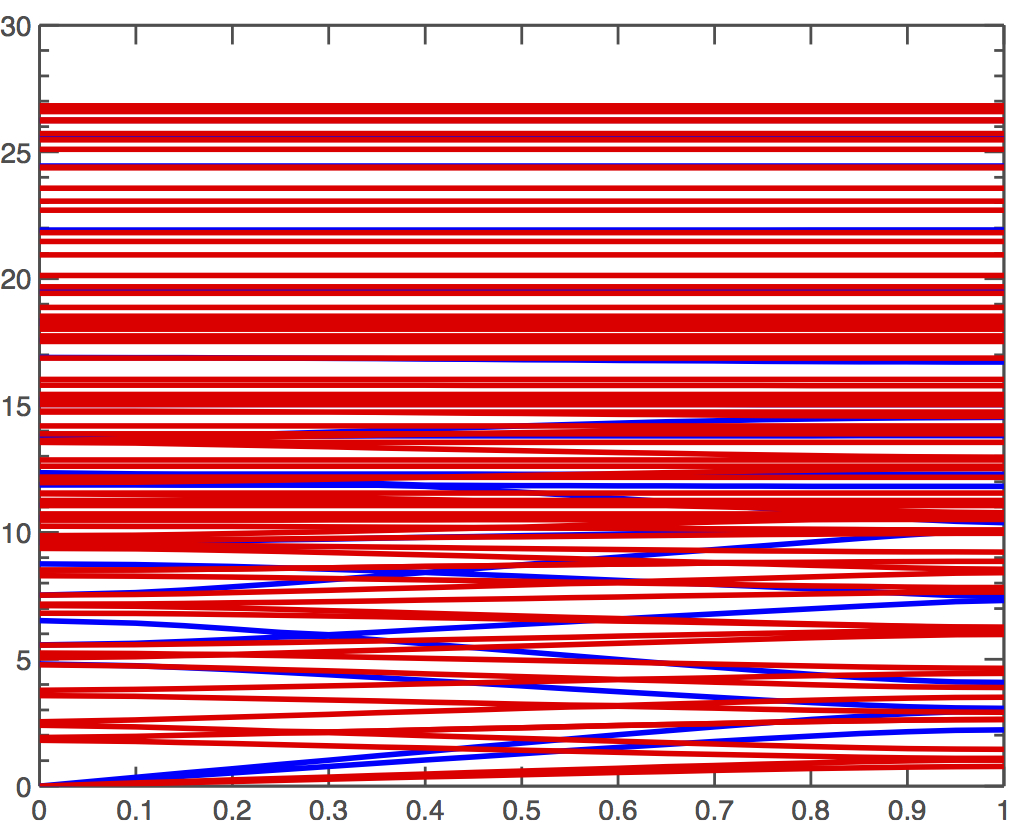
\includegraphics{dispersion.eps}}
\renewcommand{\figure}{Fig.}
\label{fig:sed}
\end{center}
\end{figure}
\begin{figure}[!h]
\vspace*{-0.8cm}
\begin{center}
\scalebox{0.48}{ \includegraphics{dispersion_ip.eps}}
\renewcommand{\figure}{Fig.}
\label{fig:dispersion}
\end{center}
\end{figure}
\end{columns}
\end{frame}


%%%%%%%%%%%%%%%%%%%%%%%%%%%%%%%%%%%%%%%%%%%%%%%%%%%%%%
%%%%%%%%%%%%%%%%%%%%%%%%%%%%%%%%%%%%%%%%%%%%%%%%%%%%%%
\subsection{Power Spectra}
\begin{frame}{Power Spectrum for $4 \times 4$}
\begin{columns}
\column{.075\textwidth}
\begin{figure}[t]
\vspace*{-1cm}
\hspace*{-0.9cm}
%\begin{center}
\includegraphics[height=70mm]{4p_dispersion_shtc_1.eps}
\renewcommand{\figure}{Fig.}
\label{fig:disp_4p}
%\end{center}
\end{figure}
\column{.91\textwidth}
\begin{figure}[t]
%\begin{center}
\vspace*{-1.2cm}
\hspace*{1.9cm}
\scalebox{0.60}{\includegraphics{sed_shtc_1.eps}}
\renewcommand{\figure}{Fig.}
\label{fig:sed}
%\end{center}
\end{figure}
\end{columns}
\end{frame}

%%%%%%%%%%%%%%%%%%%%%%%%%%%%%%%%%%%%%%%%%%%%%%%%%%%%%%
%%%%%%%%%%%%%%%%%%%%%%%%%%%%%%%%%%%%%%%%%%%%%%%%%%%%%%
\subsection{Power Spectra}
\begin{frame}{Power Spectrum for $4 \times 4$}
\begin{columns}
\column{.075\textwidth}
\begin{figure}[t]
\vspace*{-1cm}
\hspace*{-0.9cm}
%\begin{center}
\includegraphics[height=70mm]{4p_dispersion_shtc_2.eps}
\renewcommand{\figure}{Fig.}
\label{fig:disp_4p}
%\end{center}
\end{figure}
\column{.91\textwidth}
\begin{figure}[t]
%\begin{center}
\vspace*{-1.2cm}
\hspace*{1.9cm}
\scalebox{0.60}{\includegraphics{sed_shtc_2.eps}}
\renewcommand{\figure}{Fig.}
\label{fig:sed}
%\end{center}
\end{figure}
\end{columns}
\end{frame}
%%%%%%%%%%%%%%%%%%%%%%%%%%%%%%%%%%%%%%%%%%%%%%%%%%%%%%
%%%%%%%%%%%%%%%%%%%%%%%%%%%%%%%%%%%%%%%%%%%%%%%%%%%%%%
\subsection{Power Spectra}
\begin{frame}{Power Spectrum for $4 \times 4$}
\begin{columns}
\column{.075\textwidth}
\begin{figure}[t]
\vspace*{-1cm}
\hspace*{-0.9cm}
%\begin{center}
\includegraphics[height=70mm]{4p_dispersion_shtc_3.eps}
\renewcommand{\figure}{Fig.}
\label{fig:disp_4p}
%\end{center}
\end{figure}
\column{.91\textwidth}
\begin{figure}[t]
%\begin{center}
\vspace*{-1.2cm}
\hspace*{1.9cm}
\scalebox{0.60}{\includegraphics{sed_shtc_3.eps}}
\renewcommand{\figure}{Fig.}
\label{fig:sed}
%\end{center}
\end{figure}
\end{columns}
\end{frame}

%%%%%%%%%%%%%%%%%%%%%%%%%%%%%%%%%%%%%%%%%%%%%%%%%%%%%%
%%%%%%%%%%%%%%%%%%%%%%%%%%%%%%%%%%%%%%%%%%%%%%%%%%%%%%
\subsection{Perfect superlattice lifetimes}
\begin{frame}{Lifetimes}
\begin{figure}[!h]
\begin{center}
\vspace*{-0.8cm}
\hspace*{-1cm}
\scalebox{0.65}{\includegraphics{lifvomega_shtc_1.eps}}
\renewcommand{\figure}{Fig.}
\label{fig:lifetimes}
\end{center}
\end{figure}
\end{frame}
%%%%%%%%%%%%%%%%%%%%%%%%%%%%%%%%%%%%%%%%%%%%%%%%%%%%%%
%%%%%%%%%%%%%%%%%%%%%%%%%%%%%%%%%%%%%%%%%%%%%%%%%%%%%%
\subsection{Perfect superlattice lifetimes}
\begin{frame}{Lifetimes}
\begin{figure}[!h]
\begin{center}
\vspace*{-0.8cm}
\hspace*{-1cm}
\scalebox{0.65}{\includegraphics{lifvomega_shtc_2.eps}}
\renewcommand{\figure}{Fig.}
\label{fig:lifetimes}
\end{center}
\end{figure}
\end{frame}
%%%%%%%%%%%%%%%%%%%%%%%%%%%%%%%%%%%%%%%%%%%%%%%%%%%%%%
%%%%%%%%%%%%%%%%%%%%%%%%%%%%%%%%%%%%%%%%%%%%%%%%%%%%%%
\subsection{Perfect superlattice lifetimes}
\begin{frame}{Lifetimes}
\begin{figure}[!h]
\begin{center}
\vspace*{-0.8cm}
\hspace*{-1cm}
\scalebox{0.65}{\includegraphics{lifvomega_shtc_3.eps}}
\renewcommand{\figure}{Fig.}
\label{fig:lifetimes}
\end{center}
\end{figure}
\end{frame}
%%%%%%%%%%%%%%%%%%%%%%%%%%%%%%%%%%%%%%%%%%%%%%%%%%%%%%
%%%%%%%%%%%%%%%%%%%%%%%%%%%%%%%%%%%%%%%%%%%%%%%%%%%%%%
\subsection{Perfect superlattice lifetimes}
\begin{frame}{Lifetimes}
\begin{figure}[!h]
\begin{center}
\vspace*{-0.8cm}
\hspace*{-1cm}
\scalebox{0.65}{\includegraphics{lifvomega_shtc_4.eps}}
\renewcommand{\figure}{Fig.}
\label{fig:lifetimes}
\end{center}
\end{figure}
\end{frame}


%%%%%%%%%%%%%%%%%%%%%%%%%%%%%%%%%%%%%%%%%%%%%%%%%%%%%%
%%%%%%%%%%%%%%%%%%%%%%%%%%%%%%%%%%%%%%%%%%%%%%%%%%%%%%
\subsection{Bulk Lifetimes}
\begin{frame}{Lifetimes}
\begin{figure}[!h]
\begin{center}
\vspace*{-0.8cm}
\hspace*{-1cm}
\scalebox{0.65}{\includegraphics{lifvomega_defense_bulk.eps}}
\renewcommand{\figure}{Fig.}
\label{fig:lifetimes}
\end{center}
\end{figure}
\end{frame}

%%%%%%%%%%%%%%%%%%%%%%%%%%%%%%%%%%%%%%%%%%%%%%%%%%%%%%
%%%%%%%%%%%%%%%%%%%%%%%%%%%%%%%%%%%%%%%%%%%%%%%%%%%%%%
\subsection{Mixed superlattice lifetimes}
\begin{frame}{Lifetimes}
\begin{figure}[!h]
\begin{center}
\vspace*{-0.8cm}
\hspace*{-1cm}
\scalebox{0.65}{\includegraphics{lifvomega_defense_all.eps}}
\renewcommand{\figure}{Fig.}
\label{fig:lifetimes}
\end{center}
\end{figure}
\end{frame}

%%%%%%%%%%%%%%%%%%%%%%%%%%%%%%%%%%%%%%%%%%%%%%%%%%%%%%
%%%%%%%%%%%%%%%%%%%%%%%%%%%%%%%%%%%%%%%%%%%%%%%%%%%%%%
\subsection{MFP}
\begin{frame}{MFP: $\Lambda \kv=|{\pmb{\mathrm{v}}_{g}\kv}|{\tau\kv}$}
%\begin{columns}
%\column{.3\textwidth}
%$\Lambda \kv=|{\pmb{\mathrm{v}}_{g}\kv}|{\tau\kv}$
%\column{.7\textwidth}
\begin{figure}[t]
\begin{center}
\vspace*{-0.6cm}
\scalebox{0.53}{\includegraphics{MFP_cp+ip_cuml_abs_defense.eps}}
\renewcommand{\figure}{Fig.}
\label{fig:mfp_contribution}
\end{center}
\end{figure}
%\end{columns}
\end{frame}

%%%%%%%%%%%%%%%%%%%%%%%%%%%%%%%%%%%%%%%%%%%%%%%%%%%%%%
%%%%%%%%%%%%%%%%%%%%%%%%%%%%%%%%%%%%%%%%%%%%%%%%%%%%%%
\subsection{MFP}
\begin{frame}{MFP: $\Lambda \kv=|{\pmb{\mathrm{v}}_{g}\kv}|{\tau\kv}$}
%\begin{columns}
%\column{.3\textwidth}
%$\Lambda \kv=|{\pmb{\mathrm{v}}_{g}\kv}|{\tau\kv}$
%\column{.7\textwidth}
\begin{figure}[t]
\begin{center}
\vspace*{-0.6cm}
\scalebox{0.53}{\includegraphics{MFP_cp+ip_cuml_abs_defense_all.eps}}
\renewcommand{\figure}{Fig.}
\label{fig:mfp_contribution}
\end{center}
\end{figure}
%\end{columns}
\end{frame}

%%%%%%%%%%%%%%%%%%%%%%%%%%%%%%%%%%%%%%%%%%%%%%%%%%%%%%
%%%%%%%%%%%%%%%%%%%%%%%%%%%%%%%%%%%%%%%%%%%%%%%%%%%%%%
%\begin{frame}{GK}

%\begin{figure}%[H]
%\begin{center}
%\includegraphics[width=0.3\textwidth]{GK_cp5.eps} \hspace{0.05\textwidth}%
%\includegraphics[width=0.3\textwidth]{/home/schuberm/Dropbox/git/plots.nogit/images/GK_cp7.eps} \\[2em]
%\end{center}
%\end{figure}
%\column{.5\textwidth}
%\begin{figure}%[H]
%\begin{center}
%\includegraphics[width=0.3\textwidth]{/home/schuberm/Dropbox/git/plots.nogit/images/GK_cp8.eps} \hspace{0.05\textwidth}%
%\includegraphics[width=0.3\textwidth]{/home/schuberm/Dropbox/git/plots.nogit/images/GK_cp9.eps} \par
%\end{center}
%\end{figure}

%\end{frame}

%%%%%%%%%%%%%%%%%%%%%%%%%%%%%%%%%%%%%%%%%%%%%%%%%%%%%%
%%%%%%%%%%%%%%%%%%%%%%%%%%%%%%%%%%%%%%%%%%%%%%%%%%%%%%
\subsection{Thermal conductivity}
\begin{frame}{Cross-Plane Perfect SL}
\begin{figure}[t]
\begin{center}
\vspace*{-0.8cm}
\scalebox{0.75}{\includegraphics{KvL_cp.eps}}
\renewcommand{\figure}{Fig.}
\label{fig:cp}
\end{center}
\end{figure}
\end{frame}

%%%%%%%%%%%%%%%%%%%%%%%%%%%%%%%%%%%%%%%%%%%%%%%%%%%%%%
%%%%%%%%%%%%%%%%%%%%%%%%%%%%%%%%%%%%%%%%%%%%%%%%%%%%%%
\begin{frame}{Cross-Plane Mixed SL}
\begin{figure}[t]
\begin{center}
\vspace*{-0.8cm}
\scalebox{0.75}{\includegraphics{KvL_cp_all.eps}}
\renewcommand{\figure}{Fig.}
\label{fig:cp_all}
\end{center}
\end{figure}
\end{frame}

%%%%%%%%%%%%%%%%%%%%%%%%%%%%%%%%%%%%%%%%%%%%%%%%%%%%%%
%%%%%%%%%%%%%%%%%%%%%%%%%%%%%%%%%%%%%%%%%%%%%%%%%%%%%%
\begin{frame}{In-Plane Perfect SL}
\begin{figure}[t]
\begin{center}
\vspace*{-0.8cm}
\scalebox{0.75}{\includegraphics{KvL_ip.eps}}
\renewcommand{\figure}{Fig.}
\label{fig:ip}
\end{center}
\end{figure}
\end{frame}

%%%%%%%%%%%%%%%%%%%%%%%%%%%%%%%%%%%%%%%%%%%%%%%%%%%%%%
%%%%%%%%%%%%%%%%%%%%%%%%%%%%%%%%%%%%%%%%%%%%%%%%%%%%%%
\begin{frame}{In-Plane Mixed SL}
\begin{figure}[t]
\begin{center}
\vspace*{-0.8cm}
\scalebox{0.75}{\includegraphics{KvL_ip_all.eps}}
\renewcommand{\figure}{Fig.}
\label{fig:ip_all}
\end{center}
\end{figure}
\end{frame}

%%%%%%%%%%%%%%%%%%%%%%%%%%%%%%%%%%%%%%%%%%%%%%%%%%%%%%
%%%%%%%%%%%%%%%%%%%%%%%%%%%%%%%%%%%%%%%%%%%%%%%%%%%%%%
\section{Conclusions}
\begin{frame}{Conclusions}
\begin{itemize}
\item Agreement between GK and NMD for perfect superlattices
\item Agreement between Tamura theory and NMD for mixed superlattices
\item Discrepancy between GK and NMD (and Tamura theory) for mixed superlattices
\begin{itemize}
\item Mixing \textit{breaks} secondary periodicity
\end{itemize}
\end{itemize}
\end{frame}

%%%%%%%%%%%%%%%%%%%%%%%%%%%%%%%%%%%%%%%%%%%%%%%%%%%%%%
%%%%%%%%%%%%%%%%%%%%%%%%%%%%%%%%%%%%%%%%%%%%%%%%%%%%%%

%\begin{frame}{NMD vs. ALD $4 \times 4$ SL}
%\begin{figure}[t]
%\begin{center}
%\vspace*{-0.8cm}
%\scalebox{0.75}{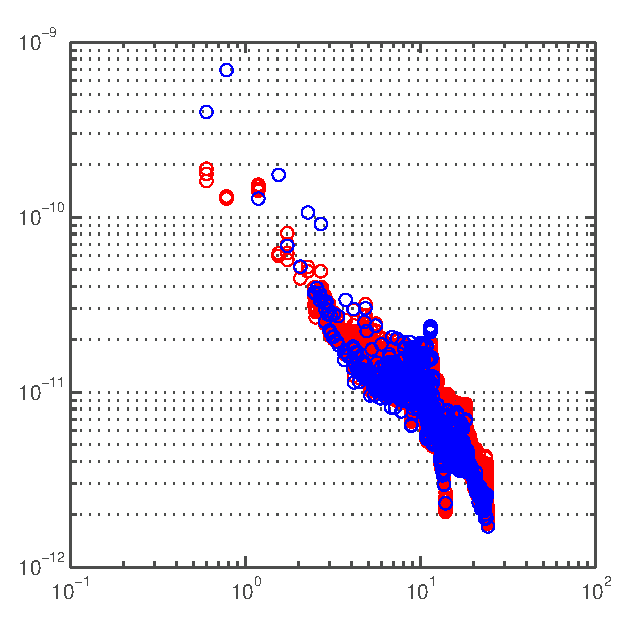
\includegraphics{NMD_v_ALD.eps}}
%\renewcommand{\figure}{Fig.}
%\label{fig:NMD_v_ALD_sl}
%\end{center}
%\end{figure}
%\end{frame}

%%%%%%%%%%%%%%%%%%%%%%%%%%%%%%%%%%%%%%%%%%%%%%%%%%%%%%
%%%%%%%%%%%%%%%%%%%%%%%%%%%%%%%%%%%%%%%%%%%%%%%%%%%%%%

%\begin{frame}{Green-Kubo}
%\begin{figure}[t]
%\begin{center}
%\vspace*{-0.8cm}
%\scalebox{0.75}{\includegraphics{GK_bulk.eps}}
%\renewcommand{\figure}{Fig.}
%\label{fig:GK_bulk}
%\end{center}
%\end{figure}
%\end{frame}

%%%%%%%%%%%%%%%%%%%%%%%%%%%%%%%%%%%%%%%%%%%%%%%%%%%%%%
%%%%%%%%%%%%%%%%%%%%%%%%%%%%%%%%%%%%%%%%%%%%%%%%%%%%%%

\begin{frame}{Size effects}
\begin{table}
\begin{tabular*}{\textwidth}{c@{\extracolsep{\fill}}ccccc}
\hline\hline\noalign{\smallskip}
Cross-Plane& \multicolumn{4}{c}{$N\times N$ Superlattice} \\
\cline{2-5}\noalign{\smallskip}
$N_xN_yN_z$ & $2\times2$ & $4\times4$ & $8\times8$ & $14\times14$  \\
\noalign{\smallskip}\hline\noalign{\smallskip}
%$4\times6\times6$ & 0.15  & 0.17  &  0.15  &  0.21 \\
$6\times6\times6$ & 0.23  & 0.22  &  0.28  &  0.36 \\
$8\times6\times6$ & 0.28  & 0.23  &  0.32  &  0.39 \\
$10\times6\times6$ & 0.29  &   &    &   \\
\hline\hline
\label{TB:K_CP_NMDsize}
\end{tabular*}
\renewcommand{\table}{Table.}
\caption{A comparison of the CP thermal conductivity NMD predictions [W/m K].}
\end{table}
\end{frame}

%%%%%%%%%%%%%%%%%%%%%%%%%%%%%%%%%%%%%%%%%%%%%%%%%%%%%%
%%%%%%%%%%%%%%%%%%%%%%%%%%%%%%%%%%%%%%%%%%%%%%%%%%%%%%

\begin{frame}{Size effects}
\begin{table}
\begin{tabular*}{\textwidth}{c@{\extracolsep{\fill}}ccccc}
\hline\hline\noalign{\smallskip}
In-Plane& \multicolumn{4}{c}{$N\times N$ Superlattice} \\
\cline{2-5}\noalign{\smallskip}
$N_xN_yN_z$ & $2\times2$ & $4\times4$ & $8\times8$ & $14\times14$  \\
\noalign{\smallskip}\hline\noalign{\smallskip}
%$4\times6\times6$ & 0.53 & 0.52  &  0.56  &  0.69 \\
$6\times6\times6$ & 0.53 & 0.51  &  0.56  &  0.59 \\
$8\times6\times6$ & 0.52 & 0.51  &  0.55  &  0.58 \\
\hline\hline
\end{tabular*}
\renewcommand{\table}{Table.}
\caption{A comparison of the IP thermal conductivity NMD predictions [W/m K].}
\label{TB:K_IP_NMDsize}
\end{table}
\end{frame}

%%%%%%%%%%%%%%%%%%%%%%%%%%%%%%%%%%%%%%%%%%%%%%%%%%%%%%
%%%%%%%%%%%%%%%%%%%%%%%%%%%%%%%%%%%%%%%%%%%%%%%%%%%%%%
\subsection{MFP}
\begin{frame}{MFP}
\begin{figure}[t]
\begin{center}
\vspace*{-0.8cm}
\scalebox{0.55}{\includegraphics{MFP_cp_defense.eps}}
\renewcommand{\figure}{Fig.}
\label{fig:mfp_contribution}
\end{center}
\end{figure}
\end{frame}

%%%%%%%%%%%%%%%%%%%%%%%%%%%%%%%%%%%%%%%%%%%%%%%%%%%%%%
%%%%%%%%%%%%%%%%%%%%%%%%%%%%%%%%%%%%%%%%%%%%%%%%%%%%%%

\begin{frame}{MD Configurations}
\begin{table}
\begin{tabular*}{\textwidth}{c@{\extracolsep{\fill}}ccccc}
\hline\hline\noalign{\smallskip}
&\multicolumn{4}{c}{Superlattice} \\
\cline{2-5}\noalign{\smallskip}
\hspace{1cm} & $2\times2$ & $4\times4$ & $8\times8$ & $14\times14$  \\
\noalign{\smallskip}\hline\noalign{\smallskip}
FFT window, $\tau_0$  & $2^{16}/2^{16}$ & $2^{16}/2^{16}$ & $2^{16}$/$2^{20}$ &$ 2^{16}$/$2^{22}$\\
Total MD timesteps & $2^{20}/2^{20}$ &  $2^{20}/2^{20}$ & $2^{20}$/$2^{20}$  & $2^{20}$/$2^{22}$\\
Number of Seeds & 5/5 &  5/5 & 5/10  &  5/10\\
\hline\hline
\end{tabular*}
\renewcommand{\table}{Table.}
\caption{Number of timesteps in the Fourier sampling windows ($\omega_H \kv \geq 1$/$\omega_H \kv < 1$), total number of MD timesteps for each superlattice system, and the total number of independent MD simulations. The use of $\omega_H\kv=1$ as the transition frequency was found to be suitable in order to obtain convergence for lifetime estimate and satisfy the $\Gamma\kv \ll \omega_H\kv$ condition.}
\label{TB:MD_time}
\end{table}

\begin{itemize}
\item The MD simulations time step is 4.285 fs (0.002 in LJ units). Equilibration is achieved by running a NVE ensemble with velocity rescaling for $1\times 10^5$ timesteps followed by a NVE ensemble for $2.5 \times10^5$ timesteps
\end{itemize}
\end{frame}

%%%%%%%%%%%%%%%%%%%%%%%%%%%%%%%%%%%%%%%%%%%%%%%%%%%%%%
%%%%%%%%%%%%%%%%%%%%%%%%%%%%%%%%%%%%%%%%%%%%%%%%%%%%%%

%\begin{frame}{Experimental Measurements}
%\begin{figure}[t]
%\begin{center}
%\vspace*{-0.8cm}
%\scalebox{0.3}{\includegraphics{experiment.jpeg}}
%\renewcommand{\figure}{Fig.}
%\label{fig:GK_bulk}
%\caption{Diagram of Frequency Domain Thermoreflectance set-up. Courtesy: Regner et al. 2013 Nature Communications}
%\end{center}
%\end{figure}
%\end{frame}

\end{document}
